\textbf{Mindmap}
Es wurde ein Brainstorm zu den Branchenspezifischen Herausforderungen und M�glichkeiten durchgef"uhrt. Das Ergebnis ist in der folgenden Mindmap dargestellt.\\

\begin{figure}[h!]
	\centering
	\caption{Mindmap Mobile Banking}
		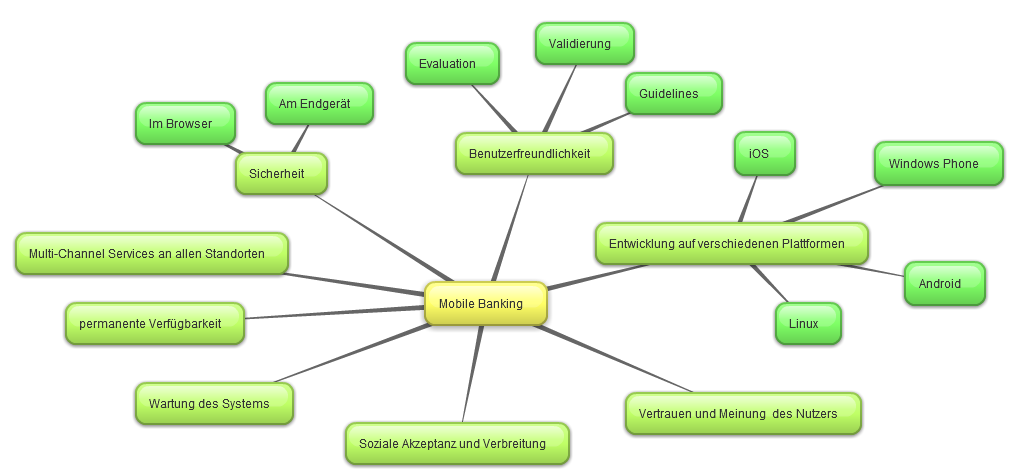
\includegraphics[width=16cm, height=10cm]{figures/mm_mobilebanking}
\end{figure}

\begin{figure}[h!]
	\centering
	\caption{Mindmap Cloud Computing}
		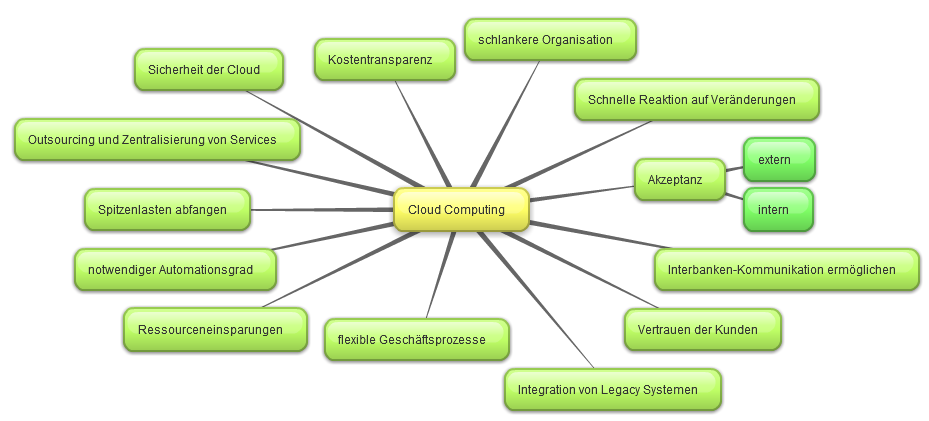
\includegraphics[width=16cm, height=9cm]{figures/mm_cloudcomputing}
\end{figure}

\begin{figure}[h!]
	\centering
	\caption{Mindmap Contactless Payment}
		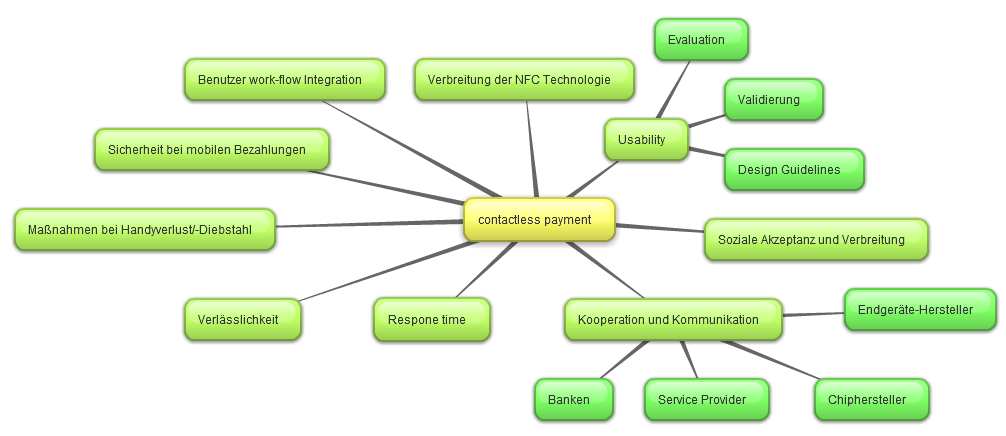
\includegraphics[width=16cm, height=9cm]{figures/mm_contactlesspayment}
\end{figure}

\newpage
\textbf{Vision \& Ziele}\\
Auf Basis der gefundenen Herausforderungen f�r das Unternehmen wurden die folgenden vier Ziele definiert welche mit einer IT-Strategie erreicht werden sollen. 

\begin{enumerate}
	\item Mobiles und intuitives Banking f�r die Kunden, anywhere and anytime.

	\item Wirtschaftliche und flexible Verwaltung von internen und externen Business-Prozessen und Produkten. 
	
	\item Aktualit"at und Innovationsf"uhrerschaft durch die Bezahltechniken von Morgen.
	
	\item Vertrauensbildung bei Kunden und Mitarbeitern zu allen Innovationen und Produkten.
	
\end{enumerate}

\textbf{Generelle Strategien}
\begin{enumerate}

	\item Einf"uhrung eines kundenfreundlichen und mobilen Banking-Portales, welches auf allen Ger�ten funktioniert und den Kunden eine breite Palette an n"utzlichen Features bietet.\\
Chris: \textcolor{red}{--> Das ist leider Falsch weil zu technisch und konkret. Kann besser in der n�chsten Sektion verwendet werden.}\\
\textbf{TBW Markus}

\begin{itemize}

	\item Chris: \textcolor{red}{Anbieten der externen Services au"serhalb der Standorte/Filialen direkt auf den Ger"aten der Kunden. -> Anywhere}
	
	\item Chris: \textcolor{red}{Durchgehende Verf"ugbarkeit von Kunden-Service, auch abseits von "Offnungszeiten. -> Anytime}	

	\item Chris: \textcolor{red}{Erh"ohung der Akzeptanz durch einfache und intuitive Nutzung der Services. Reduktion der Steuerung der Services auf das wesentliche.}		
	
	\item Chris: \textcolor{red}{Personalisiertes Nutzungserlebnis, den Pr"aferenzen und Verhalten des jeweiligen Nutzer angepasst.}	
	
\end{itemize}

	\item B"undelung von Kerngesch"aft, Kernprozessen und Kern-Knowhow. Einheitlicher unternehmensweiter Einsatz. wirtschaftliches Management von Supportprozessen. Forcieren von standortspezifischen Spezialisierungen.

	\item Bankomatkarte mit NFC Technologie ausr�sten, embedded Bankomatkarte am Handy, Partner und Vertr�ge f�r Chipkarten und Endger�te in Gesch�ften.\\
Chris: \textcolor{red}{--> Das ist leider Falsch weil zu technisch und konkret. Kann besser in der n�chsten Sektion verwendet werden.}\\
\textbf{TBW Li}

\begin{itemize}

	\item Chris: \textcolor{red}{Evaluation und Beobachtung Technischer Entwicklungen.}
	
	\item Chris: \textcolor{red}{Verfolgung und Absch"atzung von Trends und Entwicklungen sowohl im Payment-Sektor als auch in der IT.}	
	
	\item Chris: \textcolor{red}{Kn"upfen von strategischen Partnerschaften mit Markf"uhren aus dem IT und Telekommunikationssektor.}		
	
	\item Chris: \textcolor{red}{Teilnahme/Mitarbeit an relevanten Industrie-Konsortien aus dem Payment Bereich.}		
	
\end{itemize}

	\item Sicherheit, Verf"ugbarkeit und Verl"asslichkeit in allen Systemen.\\
\textbf{TBW Anton}\\
Chris: \textcolor{red}{Wichtig auch hier ist die IT-Unabh"angige Defintion.}	

\end{enumerate}









